\chapter{La machine à courant continu}
Ces machines ne sont plus utilisées comme génératrices de puissances 
mais leurs capacité de réglage de vitesse nous pousse à les étudier. 
\textbf{Dynamo} est le nom donné à une génératrice à courant continu.

\section{Génération d'une tension continue}
	\subsection{Effet d'un collecteur}
	Pour voir une f.e.m. continue, il faut 
	\begin{enumerate}
	\item Un collecteur
	\item Augmenter le nombre de conducteurs actifs
	\end{enumerate}
	Le \textbf{collecteur} est un commutateur ayant pour but de 
	redresser la f.e.m. alternative\footnote{"En électrotechnique, 
	un collecteur commutateur rotatif est un organe permettant de 
	créer 	une connexion électrique entre une partie fixe (stator) 
	et une 	partie tournante (rotor), avec une fonction de 
	commutation pendant 	la rotation. On trouve ce genre de 
	collecteur dans les machines à courant continu et les moteurs 
	électriques universels.".}.\\
	\begin{wrapfigure}[10]{l}{8.2cm}
	\vspace{-5mm}
	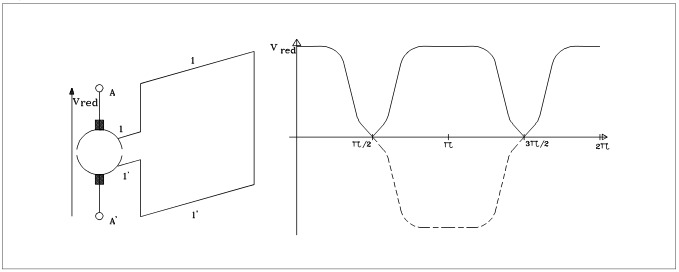
\includegraphics[scale=0.34]{ch4/image1.png}
	\captionof{figure}{ }
	\end{wrapfigure}
	\textbf{Petit plus (Source : Wikipedia) :} \textit{Ce collecteur 
	commutateur rotatif consiste en un anneau conducteur de l'électricité  
	sectionné en un nombre pair de parties 
	isolées entre elles, fixé avec une entretoise isolante sur l'axe de 
	la machine. La connexion électrique est créée entre les parties 
	conductrices et la partie fixée sur le stator (bornier), par une ou 
	plusieurs paires de balais positionnées respectivement à 180$\ ^\circ$. 
	On alimente en électricité le bobinage du rotor par ces contacts 
	(fonctionnement en moteur) ou au contraire on 	récupère l'électricité 
	produite par le bobinage du rotor (fonctionnement en générateur).}\ \\
	
	L'idée de l'espacement de $\pi$ est que le sens du courant dans 
	l'anneau conducteur va s'inverser, permettant au rotor de continuer 
	à tourner comme on peut le voir sur l'illustration ci-contre.\\
	On obtiendra aux balais une f.e.m. unidirectionnelle et dans le circuit 
	extérieur un courant unidirectionnel. Cependant, la grandeur ce cette 
	f.e.m. et du courant qui en résulte ne sont pas constantes.
	
	\newpage
	\begin{wrapfigure}[11]{r}{6.8cm}
	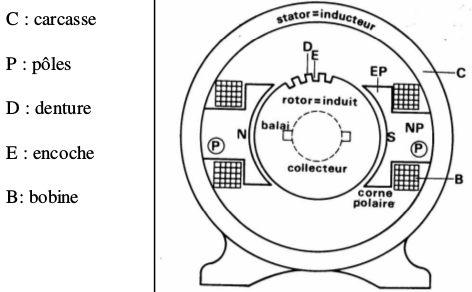
\includegraphics[scale=0.4]{ch4/image2.png}
	\captionof{figure}{ }
	\end{wrapfigure}
	Considérons un exemple "réel". Cette machine est constituée de 
	\begin{itemize}
	\item[$\bullet$] Un inducteur, sur le stator possédant $p$ paires de 
	pôles saillants. La répartition de l'induction dans l'entrefer a une 
	forme trapézoïdale avec comme axe de symétrie l'axe \textit{longitudinal} 
	$d$. L'axe électriquement $\perp$ à celui-ci est l'axe \textit{transversal},
	$q$.
	\item[$\bullet$] 	Un induit, disposés sous la forme d'enroulements de 
	conducteurs placés dans les encoches du cylindre rotorique. On connecte 
	via les faces latérales du cylindre ces conducteurs pour former un 
	\textit{enroulement en tambour.} 
	\end{itemize}\ 
	
	Les conducteurs actifs réunis par ces liaisons sont situés sous les 
	pôles opposés, d’où il résulte une addition des f.e.m. induites.
	La \textbf{commutation} d’une lame à l’autre se fait donc au moment 
	où un conducteur actif passe d’un pôle à l’autre
	
	
	\subsection{Machine multipolaire}
	On considérait jusqu'ici des machines à deux pôles inducteurs, soyons 
	fous et plaçons-en maintenant quatre. Par symétries, les f.e.m. seront 
	égales en grandeurs. Si l'on connecte les balais opposés entre eux (
	les deux négatifs ensemble, de même pour les positifs) on obtient une 
	dynamo multipolaire à \textit{enroulement parallèles}.
	
	\subsection{Types d'enroulement d'induit}
	Problème complexe non abordé ici. Sachez juste que pour l'enroulement 
	en tambour, on peut avoir l'enroulement \textit{imbriqué} ou l'
	enroulement \textit{ondulé}.
	
	\subsection{Tension à vide en régime statique}
	Soit un enroulement en tambour (l'armature, $a$) de $N_C$ conducteurs 
	répartis uniformément en deux couches. Le nombre de spires $N_S=N_C/2$. 
	On va supposer l'induit infiniment divisé de sorte à avoir une densité 
	linéique de spires $N_S/(2\pi R)$. On suppose un rotor lisse.
	
		\subsubsection{Méthode des champs}
		\begin{wrapfigure}[11]{l}{4.8cm}
		\vspace{-5mm}
		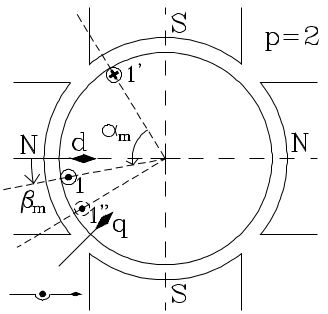
\includegraphics[scale=0.4]{ch4/image3.png}
		\captionof{figure}{ }
		\end{wrapfigure}
		Soit une spire constituée d'un conducteur d'entrée 1 et de sortie 
		1'. Nous avons
		\begin{description}
		\item[$\beta_m$ :] la coordonnée angulaire mécanique de l'entrée 1
		\item[$\beta_m-\alpha_m$ :] la coordonnée mécanique de sortie 1'
		\end{description}				
		La f.e.m. engendrée dans la spire vaut (voir figure ci-contre pour 
		la convention de signe (conducteur entrant et sortant))
		\begin{equation}
		\begin{array}{ll}
		e_{spire} &= B(\beta_m)lv - B(\beta_m-\alpha_m)lv\\
		&= (B(\beta_m)-B(\beta_m-\alpha_m))lv
		\end{array}
		\end{equation}
		Si $\alpha_m = \pi/p$ la spire est \textit{diamétrale}. Le "sens" 
		du champ $B$ sera donc exactement opposé
		\begin{equation}
		\begin{array}{l}
		B(\beta_m-\alpha_m) = - B(\beta_m)\\
		\hookrightarrow e_{spire} = 2B(\beta_m)lv
		\end{array}
		\end{equation}
		Si $\alpha_m<\pi/p$ on parle de spire \textit{à pas raccourci} : 
		on définit 1" déphasé de $\pi/p$ en avant par rapport à 1' et 
		donc déphasé de $\delta_m = \pi/p-\alpha_m$ par rapport à 1. Par 
		symétrie\footnote{??}
		\begin{equation}
		 \begin{array}{ll}
		B(1') = -B(1")\qquad\text{ou}\qquad B(\beta_m-\alpha_m) &=-B(\beta_m
		-\alpha_m+\frac{\pi}{p})\\
		&=-B(\beta_m+\delta_m)		
		\end{array}
		\end{equation}
		Impliquant que $e_{spire} = e_1-e_{1'}=e_1+e_{1"}$, en considérant 
		$B>0$ sous la pôle nord.\\
		On peut alors avoir une répartition rectangulaire de l'induction
		\begin{center}
		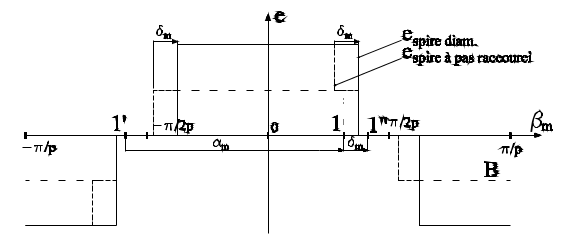
\includegraphics[scale=0.5]{ch4/image4}
		\end{center}
		ou  trapézoïdale 
		\begin{center}
		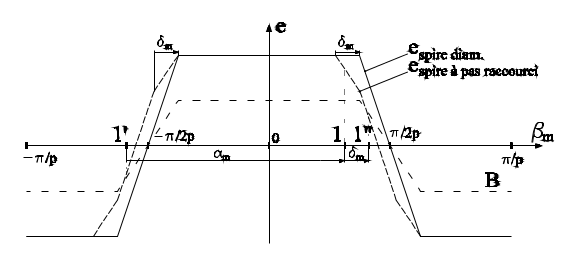
\includegraphics[scale=0.5]{ch4/image5}
		\end{center}
		
		\textsc{Forces électromotrice entre balais}\ \\
		\begin{wrapfigure}[12]{l}{6cm}
		\vspace{-2mm}
		\begin{equation}
		\begin{array}{ll}
		e &= \displaystyle p \int_{-\frac{\pi}{2p}}^{\frac{\pi}{2p}} 
		e_{spire}.\text{densité de spire}\\
		&= \displaystyle p \int_{-\frac{\pi}{2p}}^{\frac{\pi}{2p}} (
		2B(\beta_m)kv)\frac{N_s}{2d\pi}\ d\beta_m\\
		&= \displaystyle \frac{p}{d}N_s\frac{\Omega_r}{\pi} \int_{-
		\frac{\pi}{2p}}^{\frac{\pi}{2p}}B(\beta_m)lR\ d\beta_m\\
		&= \displaystyle\frac{p}{d}N_s\frac{\Omega_r}{\pi}\Phi
		\end{array}
		\end{equation}

		\end{wrapfigure}
		Supposons un enroulement à spires diamétrales tel que $e_{spire} = 
		2B(\beta_m)lv$. La f.e.m. entre balais est constante si l'induit 
		est infiniment divisé. Considérons un enroulement ondulé à $2d$ 
		dérivations : une dérivation comporte $N_S/(2d)$ spires. Celle-ci 
		est constitués par des spires dont les conducteurs d'entrée et 
		de sorties sont sous des pôles de même signe, il y a donc 
		$(N_S/2d).(1/\pi)$ spires appartenant à une dérivation par rad. 
		mécanique. Pour obtenir la tension aux bornes de la dérivation, 
		il faut intégrer les tensions de chaque spire de la dérivation. 
		Comme il y a $p$ paires de pôles, il convient de multiplier le 
		résultat d'un pôle par $p$. De façon générale :\\
		
		\retenir{\begin{equation}
		e = K\ \Omega_r\ \Phi
		\end{equation}
		où	$\Phi$ est le flux utile (coupé par une spire diamétrale 
		d'axe longitudinal de l'induit) par pôle, $\Omega_r$ en rad/s et 
		$K$, une constante qui dépend des données de l'enroulement.}
		
		\newpage
		\begin{wrapfigure}[12]{l}{4.8cm}
		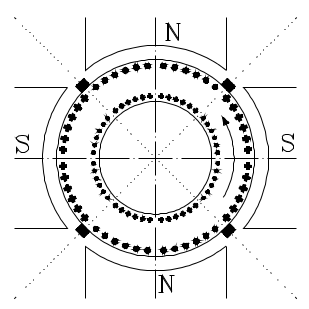
\includegraphics[scale=0.4]{ch4/image6.png}
		\captionof{figure}{ }
		\end{wrapfigure}
		La f.e.m. (tension à vide) d'une dynamo est $\propto$ au flux 
		utile par les pôles et la vitesse de rotation. Cette formule 
		reste valable pour une machine en charge ($i_a\neq0$) si on 
		considère que $\Phi$ pourrait être modifié par $i_a$. $\Phi$ 
		dépend de $i_e$ de façon non-linéaire (cf. labo).\\
		
		Ci-contre, la répartition des f.e.m. engendré pour une dynamo 
		à induit infiniment divisé de spires diamétrales. La tension 
		entre deux balais est la somme ($\int$) de toutes les f.e.m. 
		sous un même pôle. Ce schéma confirme que la f.e.m. est bien 
		alternative mais constante en un point fixe : 
		\textbf{pseudo-stationnaire} du à l'effet redresseur du 
		collecteur.

		\subsubsection{Méthode des circuits}
		
		
		
		
		
		
		
		
		
		
		
		
		
		
		
		
		
		
		
		
		
		
		
		
		
		
		
		
		
		